\newpage
\subsection*{Assignment 3.b \hrule}
\textbf{Question}
\begin{quote}
Write an interpolator for $a$, $b$ and $c$ as a function of halo mass \textbf{or} fir a function to each. Argue your specific choice! Plot the results.
\end{quote}



\textbf{Solution}
\begin{quote}

A fit should be used if the data has an error. The data is in this case approximate. A model that is fitted to the data should thus not pass through the data exactly, but should come as close as possible on average.  If the error is significant small then the data is 'exact'. In this case interpolation should be used, as an interpolator selects some kind of curve that exactly goes trough all data points and uses it to interpolate the values.

The choice of a fit or an interpolator does thus depend on the error of the data. The optimal parameters of $a$, $b$ and $c$ found by minimizing the negative log likelihood. The error for the parameters found with the downhill simplex method is atleast a function of the flatness around the minimum of the negative log likelihood.  If the negative log likelihood is flat around the minimum, then the error is larger than if the negative log likelihood is steep around the minimum. To understand this consider the following example. Let $ a = 2$, $b = 2$ and $c = 3$ be the parameters for the absolute minimum and let the negative log likelihood be flat around this minimum. The value of the negative log likelihood will for $a = 1.5$, $ b = 2$ and $c = 2.5$ be close to the value of the true parameters. The simplex will in this case have a significant amount of trouble in distinguishing the optimal values from the non optimal values. If the negative log likelihood is steep around the minimum then there is a large difference between the optimal and the non optimal variables. The simplex can in this case figure out the difference between the optimal and the non optimal values and 'walk' towards the true optimum.  


The negative log likelihood is 6 times evaluated around the found values of the minimum to check whether the error on the minimum is large or small. Let $a_{opt}$, $b_{opt}$ and $c_{opt}$ be the optimal values and let $h = 0.1$ be a small stepsize. Te negative log likelihood is then evaluated at the 6 points ($a_{opt} \pm h$, $b_{opt} \pm h$, $c_{opt} \pm h$). These 6 points are used to calculate the flatness, F,

\begin{align}
F =  \frac{1}{24 L(a_{opt}, b_{opt}, c_{opt})^2} \sum_{\text{points}} \left( L_i + L(a_{opt}, b_{opt}, c_{opt}) \right)^2
\end{align}

here $F$ is the flatness, $L(a,b,c)$ is the negative log likelihood and $L_i$ is the value of the negative log likelihood evaluated for point $i$. If $F \approx 1$, then the function is flat, else it is steep. The results after the code section show that the function is flat around the minimum for each of the mass bins. This thus suggests that a fit should be used.

\textbf{Note:} I didn't had enough time to finish this assignment. I therefore below explain what I would have done if I had enough time.

The points plotted in logarithmic space (figure \ref{fig:bleh} below the code section) shows that there might be a linear relation between the coefficients and the mass of the halo. All points are extremely flat and it is therefore assumed that all of them have the same error. A least square fit can in this case be used to fit the data with straight lines. The minimum of the least square fit can be found with one of the 1 dimensional algorithms discussed in class, or with the downhill simplex method.


The code that determines the flatness for each of the mass bins and creates the plot is located in the file: \textsf{./code/assignment3\_ b.py} \footnote{All helper functions used in this file are already shown through out this report.}. The content of the file is shown below. 
\end{quote}

\newpage

\textbf{Code - output}
\begin{quote}
The code that determines the flatness and creates the log-log point of the plot.
\lstinputlisting{./code/assignment3_b.py}
\end{quote}


\textbf{Output - text}
\begin{quote}
The found flatness coefficients. The closer the value to 1, the flatter the minimum of the negative log likelihood is.
\lstinputlisting{./output/assignment3_b_out.txt}
\end{quote}

\begin{figure}[!hb]
\vspace*{-0.5cm}
\centering
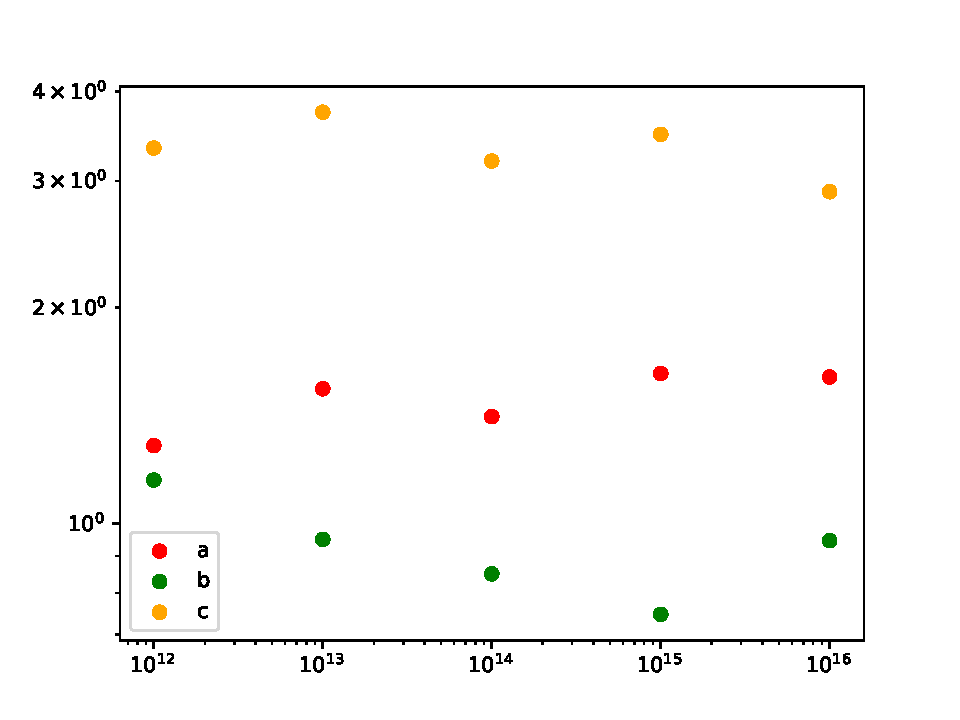
\includegraphics[scale=0.6]{plots/3b.pdf}
\caption{The optimal points plotted against the mass of the halo. The mass is in solar masses. }
\label{fig:bleh}
\end{figure}















